\documentclass[UTF8]{book}
\usepackage{graphicx}
\usepackage{caption}
\usepackage{subcaption}
\usepackage{float}
\usepackage{amsmath}
\usepackage{seqsplit}
\usepackage{tikz}
\usepackage{pgfplots}
\usepackage{listings}
\usepackage{CJK}
\newcommand\longnumber[2]{%
    \begin{minipage}{#1}
    \seqsplit{#2}
    \end{minipage}
    }
\newcommand*\thickdash{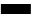
\includegraphics{thick-dash2}}
\newcommand*\thickdot{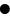
\includegraphics{thick-dot2}}

\graphicspath{ {images/} }
\begin{document}
\begin{CJK}{UTF8}{gbsn}

\title{A History of Human Communication}
\author{Dan Auerbach}
\date{2015}
\maketitle

\part{The Telegraph}

Some grabbing anecdote...

\chapter{Communication at a Distance}

Decades before the invention of the electrical telegraph that brought near-instantaneous communication to the Victorian world, the word ``telegraph'' was already in widespread use, having been coined by a French inventor named Claude Chappe to describe a network of towers that was also used to relay information. Much like signal fires that have been used since antiquity to convey simple, this \emph{optical telegraph} required no wires at all, as it instead relied on ordinary sight. In the section that follows we will explore a few different sight-based communication systems and in doing so lay some fundamental groundwork for understanding communication systems in general.

\section{Telecommunications Using Plain Sight}

Suppose you decide to play a game of catch with your friend Mary. After throwing back and forth a little, the inner athlete in Mary takes over and she decides just throwing the ball around is too boring -- she wants to practice some drills.

You're too far apart to yell at each other, so she waves you over. Soon she is excitedly describing her workout plan to you: for each throw, she is going to tell you for each throw whether she wants a high ball, or a fast line drive ball thrown hard, and your job is to deliver these balls. The point of the exercise isn't to surprise her -- she prefers to know what is coming -- but to deliver the throws she wants as accurately as possible.

You grumble to yourself about Mary's inability to just have fun without making activities so competitive, but know that it would be futile to resist. And besides, you have a much more practical question in front of you: how is she going to indicate if she wants a high ball or a low ball? After all, she's far enough away that shouting is no use. The two of you briefly consider having her hold up one finger for a high ball, and two for a low ball, but quickly realize it will be hard to discern the number of fingers she's holding up from a distance.

It doesn't take long for the two of you to devise a system. She will raise her right arm straight up in indicate that she wants a high ball thrown, and will put her right arm straight out sideways for a low ball:

\begin{figure}[H]
\centering
\captionsetup{labelformat=empty}
\begin{minipage}{.4\textwidth}
  \centering
  
\includegraphics[width=.3\linewidth]{stick-figure-arm-raised}
  \captionof{figure}{High ball}
  \label{fig:test1}
\end{minipage}%
\begin{minipage}{.4\textwidth}
  \centering
  
\includegraphics[width=.3\linewidth]{stick-figure-arm-sideways}
  \captionof{figure}{Low ball}
  \label{fig:test2}
\end{minipage}
\end{figure}

This works like a charm. Mary chooses the ball she wants, and gets to practice her catching, and you have to admit that it is kind of fun to practice particular types of throws instead of just generally playing catch.

Now, just as you are getting into a rhythm, Mary waves you over again, and your suspicions are quickly vindicated as she explains that she now wants to be able to signal one of \emph{six} different types of throws for you to deliver to her. After some grumbling, you give in and find yourself again faced with the task of coming up with a system for distinguishing the throws from one another without being able to communicate verbally.

The arm-based signaling system was working pretty well, so you decide to extend it, this time using two arms instead of one:

\begin{figure}[H]
\centering

\includegraphics{stick-figure-six-positions-simplified}
\end{figure}

It takes a little getting used to, but you pick up the system and once again settle into a rhythm, having hopefully satiated your throwing partner's lust for pushing her body to the limit. You then start to wonder if you could extend your system even further. Is there a limit to how much information you can convey with just two arms?

After thinking through it a bit more, you realize that if you could represent every letter of the alphabet via a different set of arm positions, then you could signal letters, one at a time, and communicate entire sentences back and forth. It's not too difficult to come up with such a system:

\begin{figure}[H]
\centering
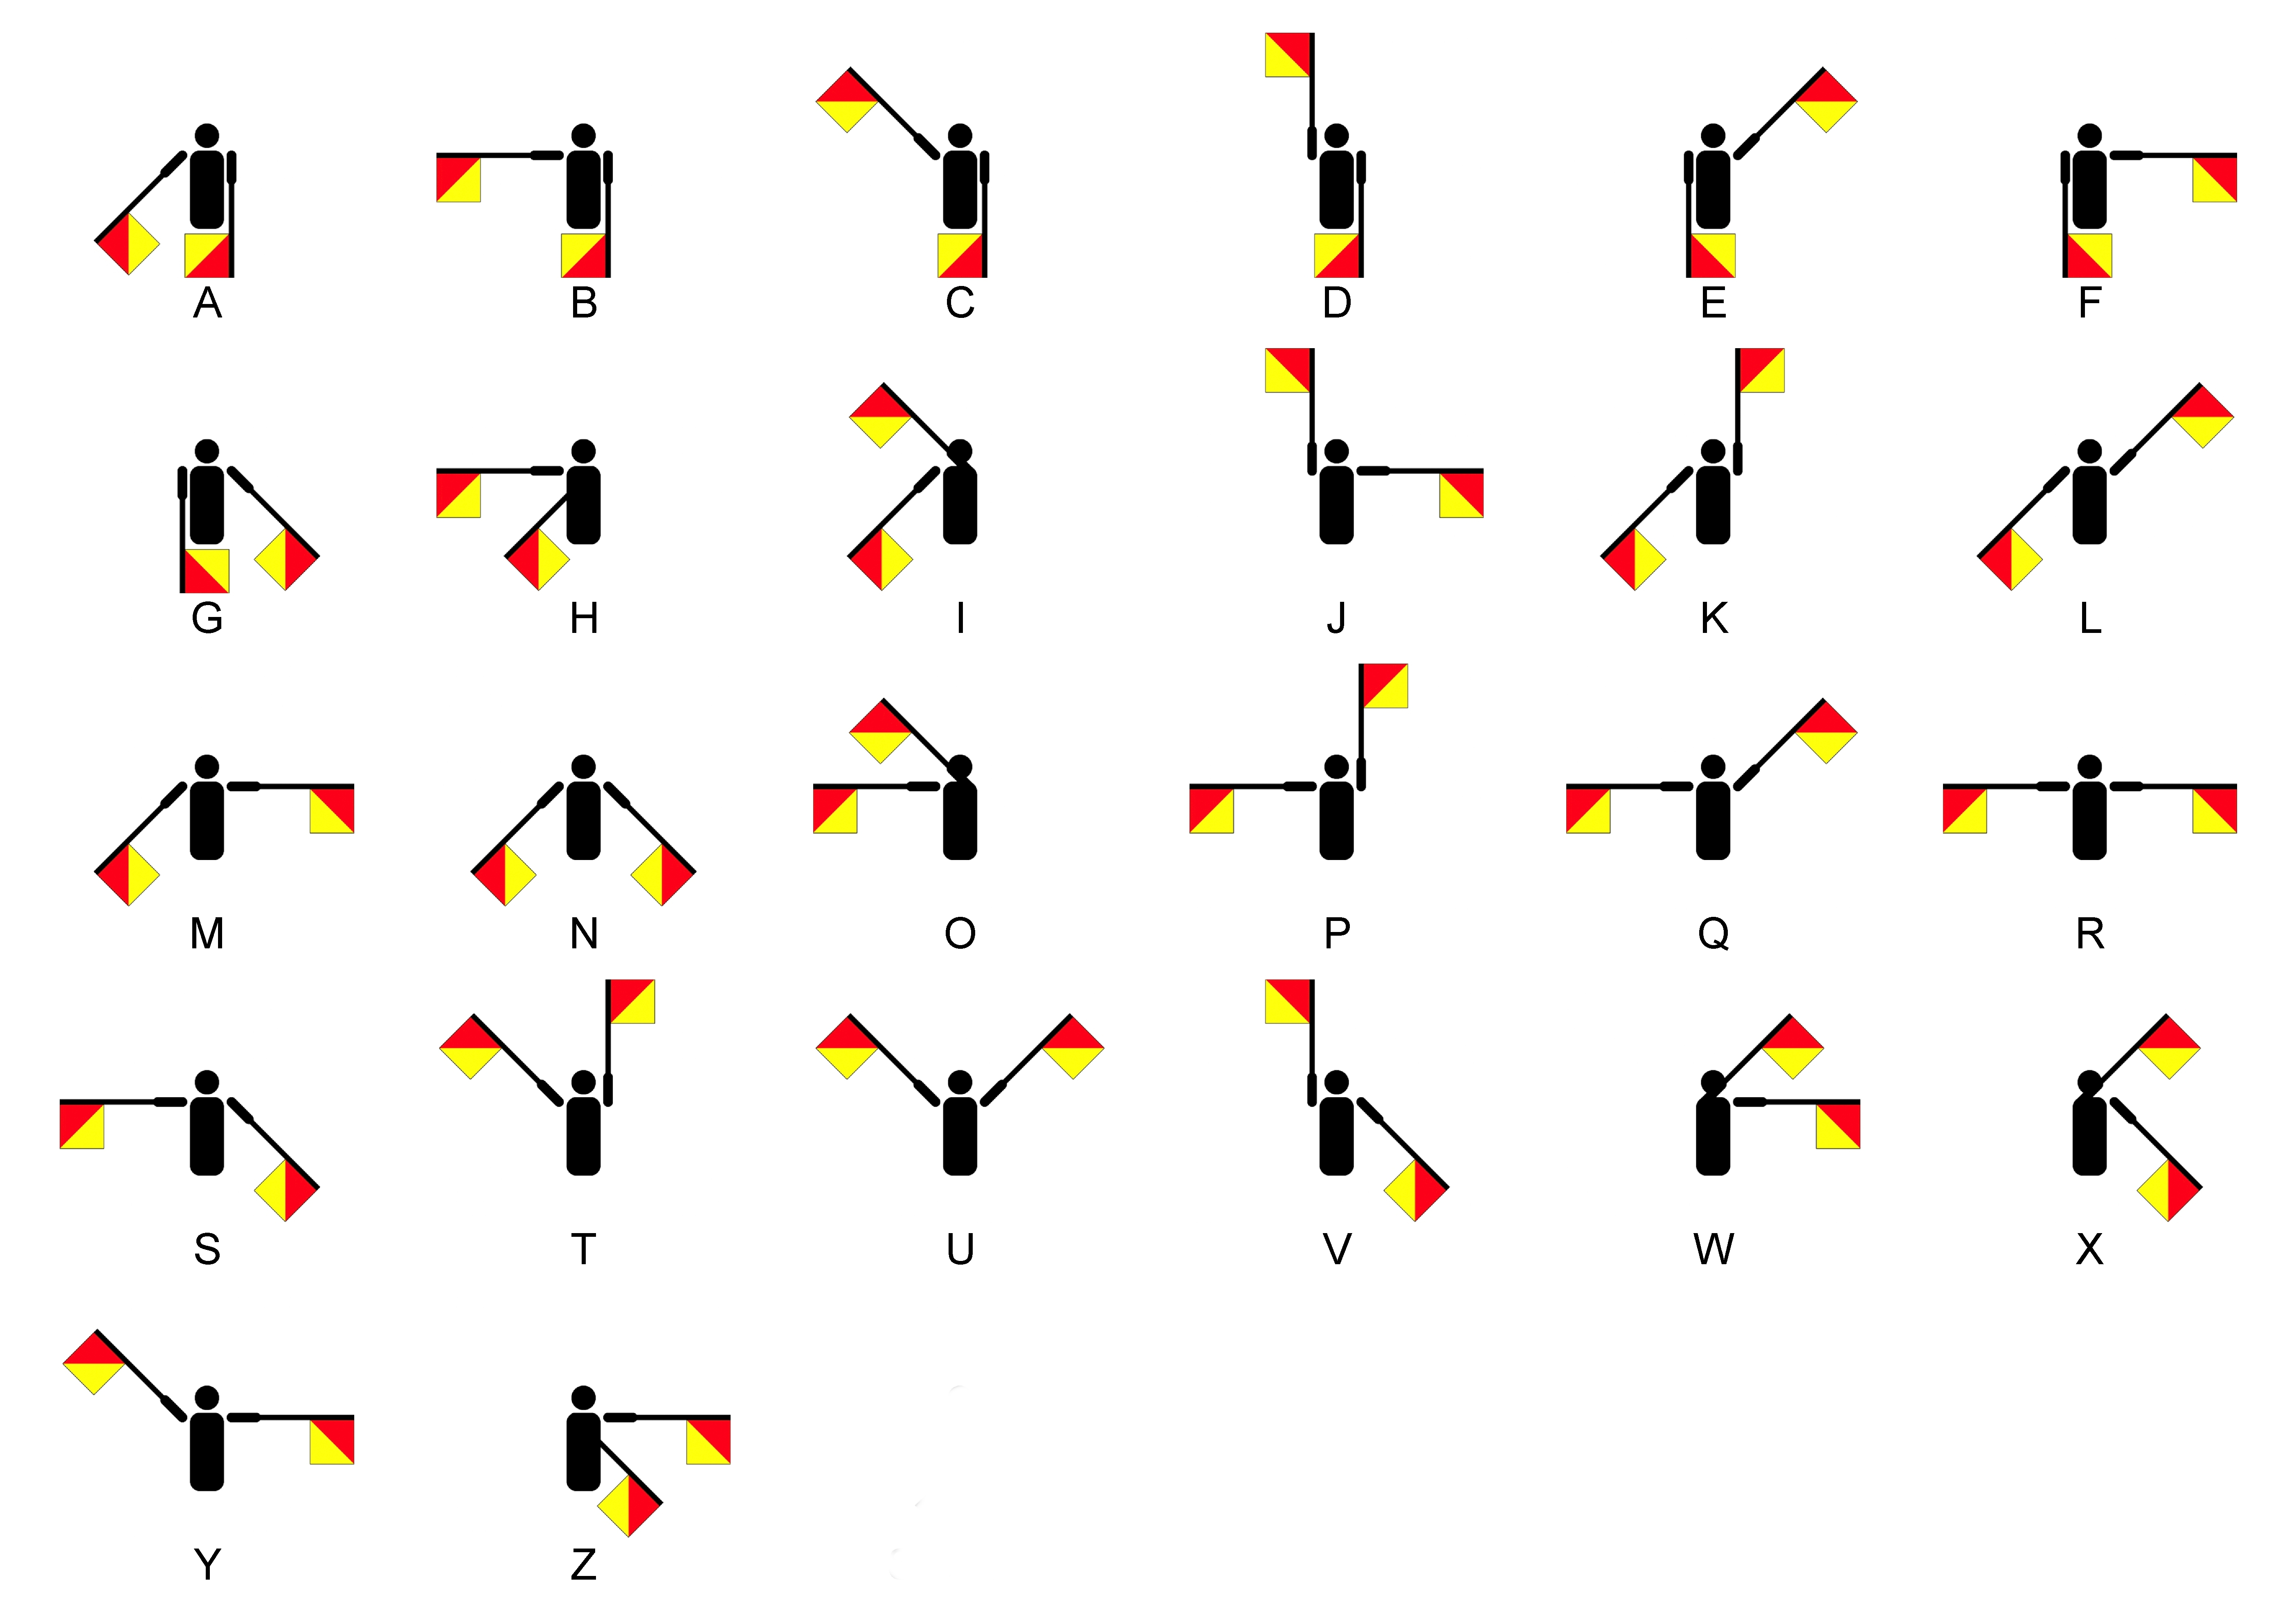
\includegraphics[width=0.9\linewidth]{semaphoreflags3}
\end{figure}

Here we display one possible system where the person signaling holds flags for extra emphasis so that the arm positions can be seen from far away.

Using this system, you could compose a message (``hey Mary, let's stop being so intense when we play catch''), and pass that message to Mary one letter at a time encoded via your arm signaling system, who in turn could decode it and understand the message.

This system is an example of what is called a \emph{semaphore system} of communication. While it may not seem that groundbreaking or useful for your game of catch, the core idea of transmitting symbols is the essence of all digital communication.

Now is there any way for us to extend this idea to quickly transfer information across dozens or even hundreds of miles?

The key insight is that to turn this basic semaphore system into something useful, we will need a \emph{network} of relay stations, each passing a message along to the next faster than any horse could ride.

\begin{figure}[H]
\centering

\includegraphics[width=0.9\linewidth]{relay_stations}
\end{figure}

Even those in the ancient world understood that relay stations could be used in this way to transmit visual information, and they did this through the creation of networks of signal fires. For example, the play \emph{Agamemnon}, which was part of a trilogy that first prize at the Dionysia festival in Athens in 458 BC, begins with a watchman looking for a signal fire that would signal the fall of Troy. [CITE]

Another famous example is African talking drums. Originating in West Africa, the instruments themselves were hourglass-shaped drums constructed to allow the player to modulate the pitch as he or she was playing. This made it possible for skilled players to approximate speech of highly tonal African languages. Even more incredible, over time sets of phrases were developed that could be played out via the talking drum and understood from far away. The phrases were intended to communicate useful information, but they had to be quite verbose so that they could be told apart from one another from a distance. For example, ``Come back home'' might be translated by the drummers into a long phrase such as: ``Make your feet come back the way they went, make your legs come back the way they went, plant your feet and your legs below, in the village which belongs to us'', which would then be ``spoken'' by the drum doing its best imitation of a person saying that phrase aloud. [CITE GLEICK]. The phrases were often relayed from village to village, forming a system of communication that could travel faster than horseback and convey complex ideas unlike signal fires.

However, both signal fires and talking drums had their shortcomings, and could not carry complex messages reliably. While other systems had been proposed to accomplish communication at a distance, it wasn't until the 1790s in revolutionary France that an inventor named Claude Chappe was able to champion and get the financial backing to build a working network capable of transmitting information. He needed a name for his new invention, and so he merged the French words for ``far'' and ``writer'', resulting in the \emph{telegraph}.

\subsection{The Chappe System}

If the idea of using a network of stations to relay information had been around for millenia, why did it take so long to start laying the stones and bricks to make it a reality?

The reasons are primarily economic. A century before Chappe was devising systems for towers to communicate, in 1684, the British thinker Robert Hooke wrote out a detailed proposal for a system of communication at a distance, but the proposal languished and was never implemented.

To get a sense of the economics at play, let's say one wanted to be able to send and receive messages from 300 miles away – roughly the distance from Paris to Lyon, or Philadelphia to Boston. Supposing intermediate stations were 10 miles apart, the cost of building the network would be the cost of building and maintaining 30 stations: that meant building 30 expensive buildings, and employing perhaps 60 human beings or more to manage the buildings and relay messages. Moreover the cost is pretty much all up front: it takes many stations to be built before information can usefully travel from large city centers.

This was too high a price for the English government of the late 17th century to spend on an unproven idea without any critical use cases. But a hundred years later when Chappe was (re)inventing his optical telegraph, revolutionary France was embroiled in intense international military conflict. In this context, not only did instability of the revolution encourage spikes in short-term spending by those in power looking out for their own interests, but the \emph{value} of being able to transmit and receive information quickly had also skyrocketed for a military waging fast-paced wars on multiple fronts.

This made the government receptive to the ideas of the young entrepreneurial Chappe, who furiously iterated on the design of his towers.

Chappe's challenge was to figure out the nitty gritty details: how were two relay stations going to actually communicate? Chappe tried a variety of systems, some rather elaborate that involved synchronizing the time between two relay stations. In the end, the simpler solution won out, a trend that we will see continues for centuries.

The relay stations would be large towers with mechanical arms that could be seen from as far away as possible. In particular, there were two small arms both connected to a large cross arm:

\begin{figure}[H]
\centering
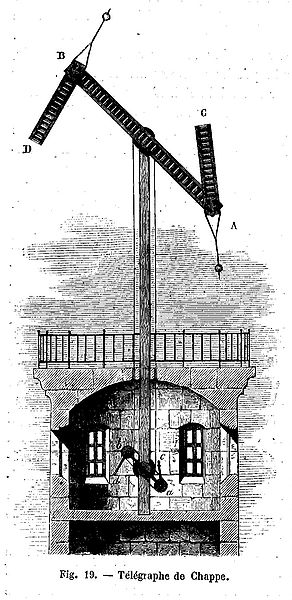
\includegraphics[width=0.3\linewidth]{chappe_tower}
\end{figure}

This obelisk was the first thing to be given the name telegraph, which we could translate as ``distant writer.'' Similar to how we used human arms when experimenting with communication earlier, the arms of the tower could be given many different positions, each corresponding to a different letter or phrase. The advantage of the mechanical arms over human ones, of course, is that the arms on the tower are much larger and hence can be seen from further away.

Since this first telegraph was to be used for strictly military purposes, the meaning of the arm positions emanating from the towers was to be kept secret. In fact, even the operators of towers often were simply mimicking the arm positions of the transmitting tower, without knowing the meaning of the message contained within that series of arm positions. [CITE]

The first line of these towers between Paris and the town of Lille was completed in 1792 and given the military usefulness, within a few years, the telegraph network spanned much of France:

\begin{figure}[H]
\centering
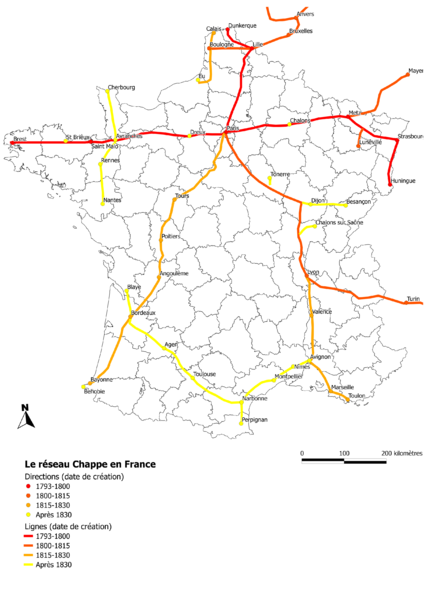
\includegraphics[width=0.5\linewidth]{chappe_network}
\end{figure}

This was the world's first extensive telecommunications (``distant communication'') network, and it required no wires at all.

The network in France was copied in other countries, as telegraph towers started appearing all over. Indeed, if you live in a hilly city, you may have a neighborhood nearby called something like \emph{telegraph hill}; this name is derived from the hills upon which optical telegraphs were placed to maximize visibility.

\section{A System of Lights}

Chappe's large mechanical arm positions provide one way to communicate effectively at a distance, mimicking the game of catch we played earlier with Mary.

In this section, let's briefly consider another method of communication using light. Suppose that your football-playing friend Mary lives several miles away on a hill which is clearly visible from your house. Just after your game of ``catch,'' as you are about to part ways, Mary extends you an open invitation to dinner for being such an excellent quarterback. She tells you to come any night that you would like -- how nice of her!

Unfortunately, there is a catch. Mary prefers a quiet life and so has no phone or Internet connection. She assures you that she will be reliably cooking every night, and that if you show up around 8 o'clock in the evening, you will be able to enjoy whatever she has prepared and there is no need to let her know in advance that you'll be joining.

But alas, you are a vegetarian, and Mary sometimes likes to cook meat. While you enjoy Mary's company, it's definitely not worth a forty five minute hike to her house unless you know Mary has cooked a meal you can enjoy.

How can Mary communicate to you so that you know whether or not to come? Building a tower is too much work, and you couldn't see it in the dark anyway.

But just as you are about to give up, Mary remembers that she has a huge bright light on her roof that when turned on is visible to you from your house. (Light bulbs were not invented until the late 1800s, so this was not available to Chappe.) If she is cooking a meal with meat, she will shine the light and leave it on all evening. That way you will know that if you see the light on, you should avoid coming over.

How does this simple communication system work? There are only two possible configurations for the light: on or off. Let's name the light being on as $1$ and the light being off as $0$:


\begin{figure}[H]
\centering
\begin{minipage}{.5\textwidth}
  \centering
  
\includegraphics[width=.5\linewidth]{house_on_hill_0}
  \captionof{figure}{``0'' (light off)}
\end{minipage}%
\begin{minipage}{.5\textwidth}
  \centering
  
\includegraphics[width=.5\linewidth]{house_on_hill_1}
  \captionof{figure}{``1'' (light on)}
\end{minipage}
\end{figure}

We can write our simple system as follows:

\begin{align*}
	0&: \text{no meat} \\
	1&: \text{meat}
\end{align*}

This works great as a system for Mary to message you about dinner, but now there's a twist -- you have a mutual friend Fred who cannot consume dairy, but does enjoy meat. In order for the system to work for both you and Fred, Mary now has to broadcast whether or not the meal being prepared that night contains meat (for you) and whether or not the meal contains dairy (for Fred). The solution is easy enough: Mary installs a second bright light, clearly distinguishable from the first. The second light is on if and only if the meal has dairy. So now when you or Fred look on Mary's house on the hill there are 4 possible configurations:

\begin{align*}
	00&: \text{no meat, no dairy} \\
	01&: \text{no meat, dairy} \\
	10&: \text{meat, no dairy} \\
	11&: \text{meat, dairy}
\end{align*}

\begin{figure}[H]
\captionsetup{labelformat=empty}
\centering
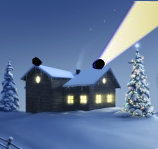
\includegraphics[width=0.25\linewidth]{house_on_hill_01}
\captionof{figure}{Example of one possible configuration ``01'' (first light off, second light on)}
\end{figure}

As we've seen, by combining 2 lights we can display 4 possible configurations. What happens when we add another friend to the mix, with an aversion to gluten? With 3 lights, how many possible configurations can we display? For each of the possible configurations we've already listed above, the third light can either be on or off, effectively doubling the number of possible configurations.

\begin{align*}
	0\quad00&: \text{no gluten, no meat, no dairy} \\
	0\quad 01&: \text{no gluten, no meat, dairy} \\
	0\quad 10&: \text{no gluten, meat, no dairy} \\
	0\quad 11&: \text{no gluten, meat, dairy} \\
          \\
	1\quad 00&: \text{gluten, no meat, no dairy} \\
	1\quad 01&: \text{gluten, no meat, dairy} \\
	1\quad 10&: \text{gluten, meat, no dairy} \\
	1\quad 11&: \text{gluten, meat, dairy}
\end{align*}

Hopefully you are starting to see a pattern. With every light we add, we double the number of possible configurations that can be displayed.

\begin{align*}
1 \text{ light} &= 2 \text{ configurations} \\
2 \text{ lights} &= 2*2 = 4 \text{ configurations} \\
3 \text{ lights} &= 2*2*2 = 8 \text{ configurations} \\
4 \text{ lights} &= 2*2*2*2 = 16 \text{ configurations} \\
5 \text{ lights} &= 2*2*2*2*2 = 32 \text{ configurations} \\
6 \text{ lights} &= 2*2*2*2*2*2 = 64 \text{ configurations} \\
7 \text{ lights} &= 2*2*2*2*2*2*2 = 128 \text{ configurations} \\
8 \text{ lights} &= 2*2*2*2*2*2*2*2 = 256 \text{ configurations} \\
9 \text{ lights} &= 2*2*2*2*2*2*2*2*2 = 512 \text{ configurations} \\
&\text{etc}
\end{align*}

Written more concisely, we have just seen that if we have some number $n$ lights, then we can display $2^n$ possible configurations.

There are many more questions we might want to answer about our system of lights. What messages can be sent with these lights? What about just a single light? How fast can information be transmitted? What if a light is burned out? We will return to these questions in time, but first let's travel back to the early 1800s, when people were only first starting to understand the power of electricity.

\chapter{The Electrical Telegraph}

So far we've talked about two systems for communicating at a distance: the optical telegraph system, and the system of lights on top of Mary's house. One major limitation of both of those systems is that they rely on line of sight. What happens if it gets foggy? Or if you want to communicate across a large body of water that doesn't allow for the construction of towers along the way?

The electrical telegraph solves these problems, providing a more robust solution to long distance communication. Electricity can be made to travel over a wire and this can in turn be used as the fundamental building block of a communication system. This approach doesn't have the shortcoming of the line-of-sight approaches – the wires can snake around large mountains, treacherous deserts, and lie at the bottom of bodies of water. Moreover, electrical telegraphy doesn't require expensive towers to be built and maintained, and wires can fairly easily be repositioned, and so a network based on the electrical telegraph is much less expensive and more flexible than an optical telegraph network.

Given all the advantages of the electrical telegraph, it is no surprise that shortly after being invented, it eclipsed the optical telegraph as the dominant mechanism for communicating at a distance, and nowadays when someone talks about the ``telegraph'' they are almost certainly referring to the electrical telegraph. I will follow this convention, and explicitly use the phrase ``optical telegraph'' when I need to refer to the older line-of-sight-based Chappe technology.

The development of the electrical telegraph occurred in the first half of the 19th century, and relied on advances in battery technology and a steady progression in our ability as human beings to harness the power of electricity in increasingly sophisticated ways. The telegraph in some sense represents society's first proof of the power of electricity, since it is by most measures the first major technology based on electricity that ordinary people interacted with on a regular basis.

Like many great inventions, the ideas behind the telegraph were developed more or less independently by more than one person, and bitter patent lawsuits were not far behind. The man who has ended up getting the majority of the credit as the father of the telegraph is Samuel Morse, an American painter-turned-inventor who was born in 1792, right when Chappe was furiously iterating on his towers. Morse was unaware of telegraphy of any sort through his early life; he painted portraits through his 30s and only in his 40s turned his attention towards electricity and the idea of creating a system of communication using electricity over a wire. He then obsessively worked on this problem until he eventually developed and popularized the dominant telegraphy system which became the standard for the next sixty years.

Besides Morse, the other prominent pair of inventors were Cooke and Wheatstone, who worked in England, independently developing their own ideas and systems for how to communicate over a wire. Conceptually, all of these people were on a similar track, but Morse's system had certain advantages over that of Cooke and Wheatstone, and eventually even Cooke and Wheatstone agreed that the ``Morse system'' was superior.

\section{A Simple Circuit}

An electric telegraph is in essence just a very simple electrical circuit. There is a power source, a switch and a loop of wire connected to an electrical device that acts as a receiver indicating whether or not electricity is flowing through the circuit:

\begin{figure}[H]
\centering
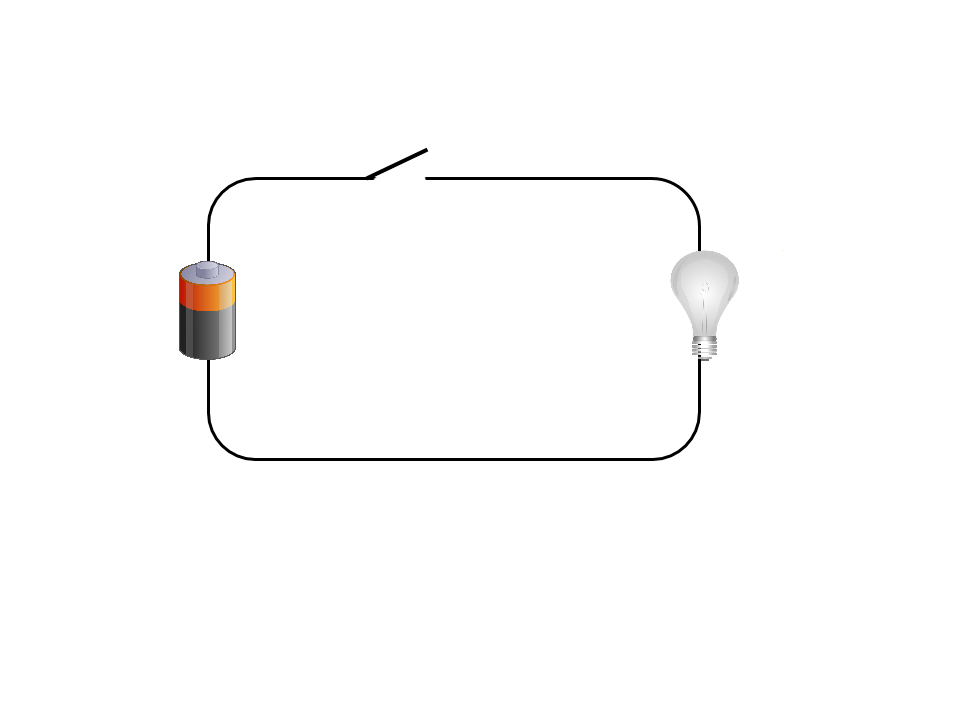
\includegraphics[width=0.8\linewidth]{circuit1}
\caption{Switch closed; no electrical current}
\end{figure}


In the circuit diagram above, the power source is the battery is drawn on the left. It has positive and negative terminals, which we'll talk about in a minute. The little angled line represents a switch. If the switch is open, as it is in the diagram above, electricity does not flow through the circuit. If the switch it closed, on the other hand, then an electric current flows through:

\begin{figure}[H]
\centering
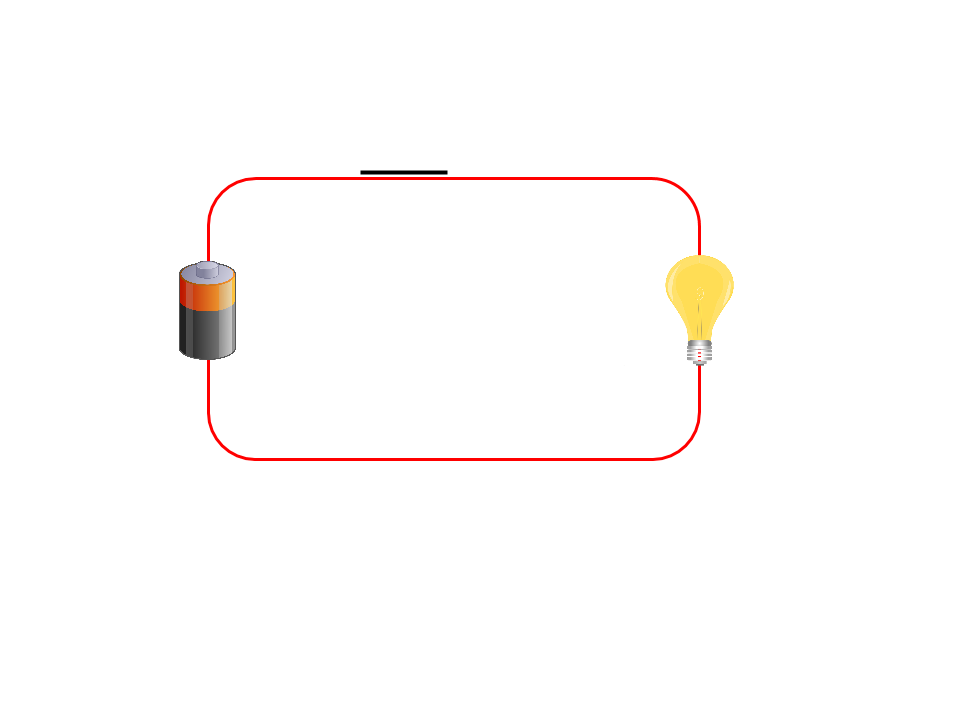
\includegraphics[width=0.8\linewidth]{circuit2}
\caption{Switch open; electricity flowing}
\end{figure}

When electrical current flows through the circuit, the electrical device on the right hand side has electricity running through it. Typically in elementary electrical engineering textbooks, a lightbulb is used as an illustration of this electrical device indicating that electricity is flowing through a circuit.

Unfortunately for Morse and his peers, there were no light bulbs in the 1830s and 1840s, but there were elementary alternatives serving the same conceptual function as a light bulb.

\section{One Telegraph to Rule Them All}

While all electrical telegraphy developed through the 1840s was based on the paradigm of a simple circuit that we described above, the details varied quite a bit among competing designs. There was not a single telegraph during this period, but rather a plethora of distinct competing experimental systems for communicating over electrical wires.

Many early designs involved creating one circuit per letter of the alphabet. In England in the late 1830s, Cooke and Wheatstone developed a working prototype of a telegraph that involved six wires. On the receiving end of this telegraph, there were five needles that could be made point to a particular letter:

\begin{figure}[H]
\centering
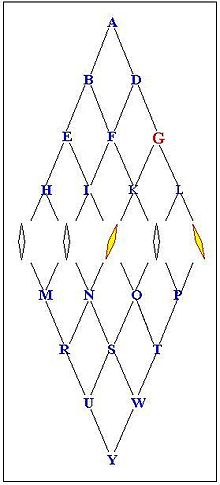
\includegraphics[width=0.4\linewidth]{wheatstone}
\caption{Cooke and Wheatstone telegraph needles pointing at 'G'}
\end{figure}

When the dust settled, however, the telegraph that became the de facto worldwide standard was an iteration coming from Morse and his collaborators, notably Alfred Vail. As we will see time and time again, simplicity is a major virtue when designing a telecommunications system, and this was an advantage of the Morse telegraph over other early prototypes.

Let's look in a bit more detail at how the Morse telegraph worked. Here is a representation superimposed on our basic circuit above:

\begin{figure}[H]
\centering
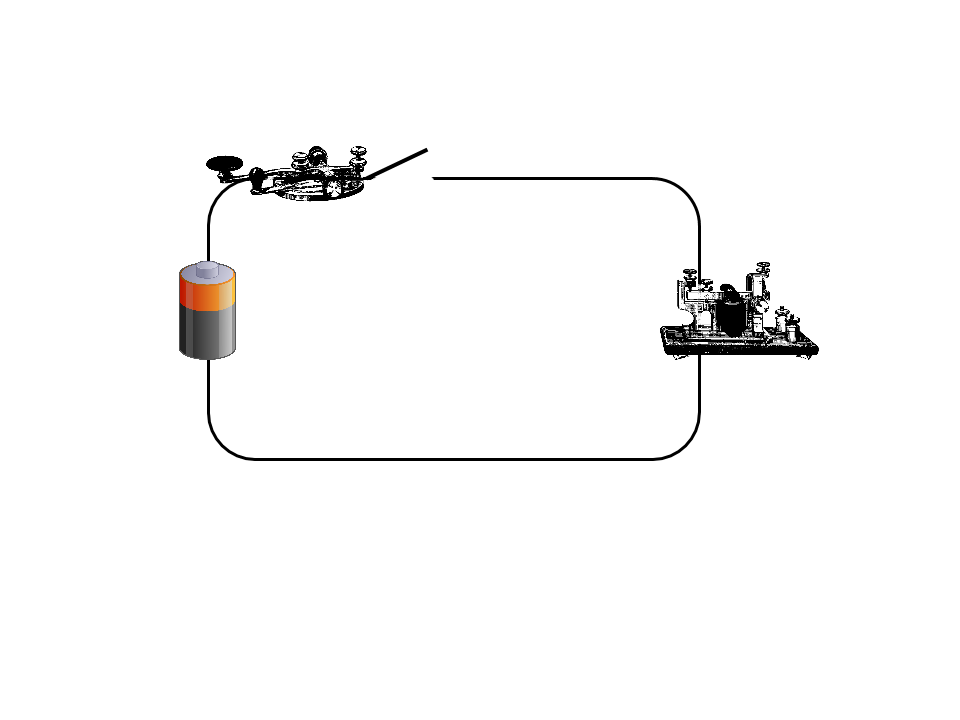
\includegraphics[width=0.8\linewidth]{telegraph_as_circuit}
\caption{Telegraph as a basic circuit}
\end{figure}

The circuit was closed by default, which means that electricity was flowing through. Transmission occurred via \emph{telegraph key}, an invention of Vail that was essentially just a single button that an operator could press. When pressed, the circuit was opened and electricity no longer could flow through the wire. When released, electricity resumed.

\begin{figure}[H]
\centering
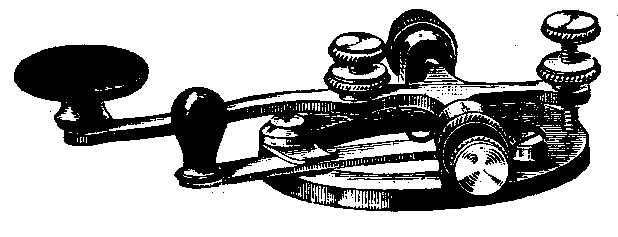
\includegraphics[width=1.0\linewidth]{telegraphkey}
\caption{Telegraph key}
\end{figure}

Telegraph operators would tap out messages with this single key in a specified manner (which we'll discuss shortly).

On the receiving end, there was a bit more variance in terms of what gadget was actually used to receive messages over the life of the telegraph. After experimentation with all sorts of receiving devices –- making little marks on paper, making needles point to particular locations, and so on -- the winning gadget employed throughout the peak of the telegraph in the mid to late 1800s was called a \emph{sounder}:

\begin{figure}[H]
\centering
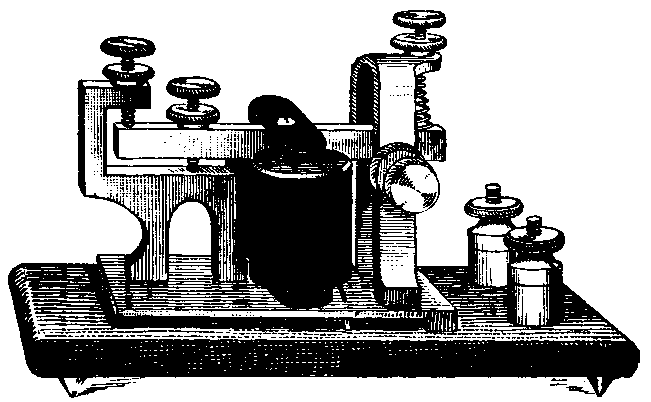
\includegraphics[width=0.8\linewidth]{telegraphsounder}
\caption{Sounder}
\end{figure}


This device allowed telegraph operators to listen to clicks and pauses which corresponded to the pressing and lifting of the telegraph key by the operator at the other end of the line. So we now have a clearer picture of how a telegraph worked: it was essentially a circuit with a key on one end corresponding to a switch and a sounder on the other end that allowed key presses to be heard as clicks.

\section{Morse Code}

Knowing that someone on the other end of a telegraph line hundreds or thousands of miles away is pressing a key at this very moment is a remarkable achievement, but in order for it to be useful for communication, there needs to exist a \emph{system} that translates the ``on'' and ``off'' states of the telegraph into useful information.

We've discussed a couple such systems already, but these relied on line of sight and being able to display lots of information at once, either in the form of varying arm positions or in various lights that are on or off. In this case, we only have a single on or off state that varies over time. How can this be used to convey information?

The system that stuck for telegraphy is known as Morse code. Morse code enables communication by segmenting the raw ``on'' and ``off'' states into four symbols: a dot, a dash, a short pause, and a long pause. A short press of the telegraph key was called a ``dot'' and a long press of the key was called a ``dash''. Different lengths of pauses were necessary to differentiate a pause between letters from a pause between words.

\begin{center}
\begin{tabular}{cc}
\thickdot & dot \\
\hline
\thickdash & dash \\
\hline
[short pause] & letter space \\
\hline
[long pause] & word space \\
\end{tabular}
\end{center}

These four symbols comprise the basic alphabet of telegraphy, but we also need a way to translate this basic alphabet into English letters, much as we did for our system of lights earlier. It is not too difficult to create such a table:

\begin{figure}[H]
\centering
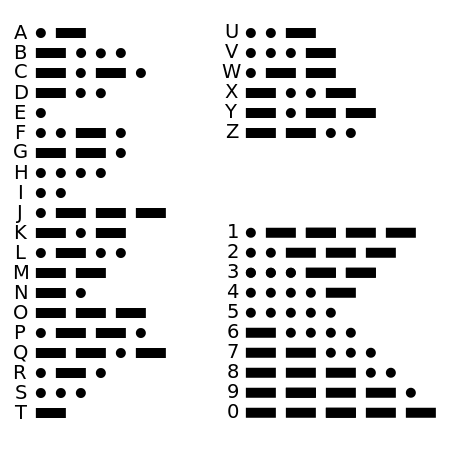
\includegraphics[width=0.8\linewidth]{morse-code}
\caption{International Morse Code standard}
\end{figure}


Armed with this system, the telegraph is transformed from a meaningless single-signal transmission device into the world's first widespread telecommunication technology. The way it works is similar to the semaphore system we outlined above. For example, consider the following sets of dots, dashes, short pauses and long pauses, represented on paper via our table above:

\[ \thickdot \thickdot \thickdot \thickdot \quad \thickdot \quad \thickdot \thickdash \thickdot \thickdot \quad \thickdot \thickdash \thickdot \thickdot \quad \thickdash \thickdash \thickdash \]

Using the translation table, this would correspond to the English word:

\[ \text{Hello} \]

The Morse system has the advantage that only a single circuit is needed to communicate, meaning that even very simple designs for the physical telegraph could be made to effectively communicate via Morse code. In particular, unlike the more complex designs of Cooke and Wheatstone (as well as Morse's earlier systems), the telegraph which became the standard did not require several wires across multiple circuits to be synchronized, cutting down the complexity and cost of the system significantly.

\section{Practical Limits of Telegraphy}

We now have a basic high level understanding of how the telegraph works, but before dismissing this topic as fully understood, it's worth pausing to reflect on all of the unknowns that we would need to flesh out to have a complete understanding of the telegraph.

Perhaps the largest looming question is how electricity works. We will cover this topic in more detail in the next part of this book, so if you aren't already knowledgeable on electromagnetism, I encourage you for now to rely on a high level understanding of electricity as the flow of free electrons through wires made from conducting metals like copper. Electricity has a current, like a river, and moves very fast.

This very rough notion approximates the mentality of engineers through the 1850s (minus knowing about electrons), since it wasn't until later in the 19th century that James Clerk Maxwell and others paved the way for our contemporary understanding of electromagnetism.

Despite a lack of theoretical understanding of the fundamental principles that enabled electrical telegraphy to function, it did manage to work nevertheless. But it didn't work perfectly, and so a lot of energy was spend trying to get telegraphs to be more reliable, to function over long distances, and to be able to cross harsh terrain.

One challenge at first seemed insurmountable: could a telegraph cable be built that traversed the Atlantic ocean?

To achieve this, improvements to cabling were critical. In particular, early telegraph systems involved stringing raw copper wire along poles, or burying it underground. But raw copper wire was super unreliable as a transport mechanism: it could be easily damaged, and simply did not work that well (a lot of which can be chalked up, in retrospect, to electrical interference).

So for telegraphs to function at scale, more sophisticated cabling was needed. Fortunately, \emph{gutta-percha} was discovered by the industrial world in 1843 and quickly became a household name in the Victorian world. This tree sap known for producing a naturally rigid latex became the mid to late 19th century's equivalent of plastic today, and among its myriad uses was as an insulator surrounding raw copper telegraph wires. The gutta-percha in turn was often wrapped in rubber, and then an outer layer or iron or steel, creating a cable whose cross section looked like this:

\begin{figure}[H]
\centering
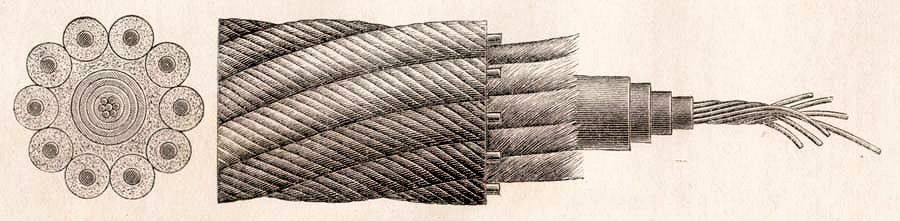
\includegraphics[width=0.8\linewidth]{cable-cross-section}
\caption{Telegraph cable}
\end{figure}

It did not happen overnight, but 14 years after Morse's first successful proof of concept of the electrical telegraph in 1844 between Baltimore and Washington, D.C., the first transatlantic telegraph cable was laid, ushering in the dawn of a new information age of instantaneous cross-continent communication.

In addition to better cabling, there were a lot of open questions. How thick should the copper wire be? How powerful should the battery be? The engineers involved in these early projects engaged in a tremendous amount of trial and error, and succeeded in pushing the range and reliability of telegraph lines despite very little theoretical understanding of electricity and magnetism.

Yet even as engineers inched towards cables that were better optimized for the task at hand, there remained one unfortunate fact of life: over longer and longer distances, the strength of the signal diminished.

This phenomenon, which in contemporary parlance is called \emph{attenuation} of the electrical signal, is due to the fact that energy is lost when electricity travels over a wire. To solve the fact that the signal would get weaker over longer distances, some sort of repeating mechanism was needed.

\section{Electromagnets and Relays}

Underlying the repeating mechanism is a fundamental electrical device called an \emph{electromagnet}, first invented in the 1820s.

You can think of a simple electromagnet as a piece of iron with insulated wire tightly coiled around it:

\begin{figure}[H]
\centering
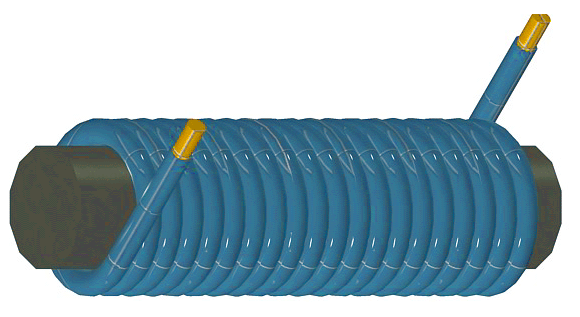
\includegraphics[width=0.8\linewidth]{electromagnet}
\caption{Simple electromagnet}
\end{figure}

When current flows through the wire, it induces a magnetic field, making the iron into a magnet. This allows the flow of electricity to dictate whether a magnet is ``on'' or ``off''.

One of the reasons the electromagnet is so important is that it allows electrical current to create mechanical action. To see how this is possible, consider the following setup:

\[ [DIAGRAM] \]

When electricity flows, the electromagnet is activated, creating a magnetic field, which pulls the metal latch down. When the flow of electricity stops, the magnetic field disappears and the latch returns to its original position.

\[ [DIAGRAM] \]

Now what if the metal latch that is going up and down is actually the switch of another electrical circuit? You can now have two circuits with independent power sources linked by this electromagnet like this:

\[ [DIAGRAM] \]

An electromagnet used in this way is called a \emph{relay}. Imagine the left side of the above diagram as a telegraph operator using a telegraph key. When the operator presses down, communicating a dot in Morse code, it opens the switch and cuts the electrical current for a brief moment. This causes the magnetic field to disappear in the electromagnet, and so the latch in the relay returns to it's original position, which breaks the current on the right hand side, communicating a dot.

By offering a way around the signal attenuation issue, relays allowed telegraph lines to extend arbitrarily far, though of course relays were yet another piece of equipment that had to be installed and maintained. Still, compared to the Chappe optical telegraph system, in which the ``repeaters'' were actually just human beings re-coding the message, electrical relays are a huge cost savings.

Electromagnets had another important purpose. Recall that a sounder was used at the receiving end of telegraphs to listen to the dots and dashes of Morse code. But how did a sounder actually work? It was an electromagnet that worked just like a relay, except that instead of controlling another circuit, the latch going up and down made respective and distinct ``click'' and ``clack'' sounds, allowing operators to identify difference cadences of clicks and clacks with the Morse code alphabet, which they could in turn decode into English.

\chapter{A Layered Symbolic System}

The telegraph was in one important way a direct precursor to the Internet. Unlike the analog telephone and broadcast radio and television technologies that succeeded it, the telegraph was a \emph{digital} communication system and in this respect strangely ahead of its time. To understand why, we must look a bit more abstractly at symbols and information.

\section{Alphabets and Symbols}

Consider the letter \emph{`a'}, the first letter of the Latin alphabet. What makes this mark meaningful? If we did not know English or any other languages based on this alphabet, then \emph{a} would just appear to be a mysterious mark with no meaning, such as $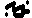
\includegraphics{randomsymbol}$.

Thus for the letter \emph{a} to carry information for the onlooker, it has to exist within the context of what we can call an \emph{alphabet}. And of course, the Latin alphabet is not the only meaningful alphabet. The traditional Chinese character 章 may look meaningless to a non-Chinese reader, but it certainly has a meaning within the context of the traditional Chinese alphabet.

What about a number like \emph{2}? You might think that this is not part of an alphabet, since it is a number and not a letter. However, for our purposes, we are intentionally going to use the word \emph{alphabet} very broadly, as mathematicians do, and by this broad definition, the symbols 0, 1, 2, 3, 4, 5, 6, 7, 8, 9 do indeed form an alphabet which we usually call Arabic numerals. Just think of an alphabet as any fixed set of symbols that are distinguished from one another by some known rules or conventions.

There are some interesting edge cases. For example, consider the following set of symbols:

\begin{figure}[H]
\centering
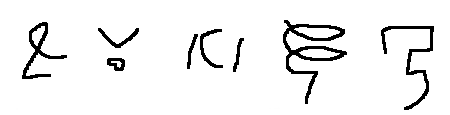
\includegraphics[width=0.8\linewidth]{random-symbols}
\caption{Set of symbols}
\end{figure}

Does this form an alphabet? The symbols have no meaning in themselves, but I just wrote them down and said that they ought to be go together. Is that enough to constitute an alphabet? Does there have to be some sort of shared knowledge of more than one person, or generally accepted use for the symbols of the alphabet? Or can one create a bare ones alphabet by fiat, as I just did above?

Another edge case occurs when we consider infinite alphabets, like:

\begin{figure}[H]
\centering
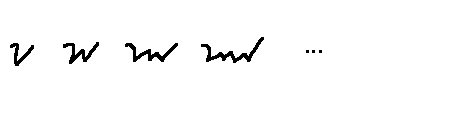
\includegraphics[width=0.8\linewidth]{infinite-alphabet}
\caption{Infinite alphabet}
\end{figure}

Does this count as an alphabet? One interesting question that arises here: do symbols have to be specified explicitly at the outset when defining an alphabet, or is it enough to describe how one \emph{could} draw the symbols, for example by giving a schema for the user of the alphabet to fill in?

With a little bit of math, one can create a formal definition of alphabet and in doing so start to better understand these unusual examples. Fortunately for our purposes, the important thing is not the edge cases or formal definition, but rather just a basic understanding of an alphabet as a backdrop against which sets of symbols have meaning.

That's enough to come to our first major insight about symbols and alphabets: all symbolic representations are interchangeable.

What does this mean? If you fix a translation system, you can take any string of symbols from one alphabet and translate using the agreed upon translation system to any other string of symbols in another alphabet.

As an example, consider the sentence:

\begin{quotation}
\centering
\emph{All symbolic representations of information are fungible!}
\end{quotation}

For starters, we could translate this to the traditional Chinese alphabet, giving us a new representation of the sentence:

\begin{quotation}
\centering
\emph{所有的信息符號表示是可替代的!}
\end{quotation}

I mentioned above that one had to agree on a translation system.  Which one was employed for this translation? We might call it a \emph{semantic} translation system, in that the underlying meaning of the sentence was recreated via a new sentence in Chinese. This is actually a tremendously difficult and complicated translation system. Fortunately, we can also come up with much simpler translation systems.

To see this, let's translate the above sentence into Arabic numerals. \emph{Guh? How can you translate a sentence into numbers!?} The important thing to remember is that we get to decide on the translation system. In this case, we can pick something arbitrarily, just like we did earlier during our game of catch with Mary. Let's just translate each letter to it's position in the alphabet:

\begin{quotation}
\centering
\emph{1 12 12  19 25 13 2 15 12 9 3  18 5 16 18 5 19 5 14 20 1 20 9 15 14 19  15 6  9 14 6 15 18 13 1 20 9 15 14  1 18 5  6 21 14 7 9 2 12 5 !}
\end{quotation}

This \emph{almost} counts as a translation into the 10-symbol Arabic alphabet that we specified above. But there is a subtle issue that we need to deal with: we still have whitespace characters and the `!' character, neither of which occur in the Arabic alphabet. You might counter that neither of these are considered part of the 26-character Latin alphabet that underlies English. But remember that we are using the word alphabet in a particular sense, and in this sense, any alphabet that underlies ordinary written English must have symbols corresponding to whitespace and exclamation points, since these are part of the language. Put another way, if we formalize the written English language as a system for communication, it will include extra conventions beyond the Latin letters one learns in elementary school; whitespace is part of the language too and the easiest way to capture it the rules around whitespace is to say that there is a `space' character.

Hence, to make our mapping to the alphabet of Arabic numerals a proper translation, we need a way to separate the words without using the space or exclamation point characters, neither of which we are allowed to use in our new alphabet. This isn't as trivial as simply removing the characters, since we need to away to disambiguate strings like '15' which could be either `af' or `p'.

We also need this character separator to be some sort of number, in other words a string of one or more digits from 0 to 9. We didn't use the symbol `0' for any English letter, and it is available to us, so how about that? That almost works, except that there are still some ambiguous strings. For example, `2002' could translate into `b  b' or `t b'. We're getting closer, though. The problem with our current system that creates the above ambiguity is that each English letter could correspond to a variable number of digits. What if instead we enforce that every letter is exactly two digits long, so the letter 'a' is actually '01'? Now we can make '00' a space, and '27' an exclamation point. Moreover, we can also encode upper case letters and other common symbols as a sequence of two digits. Here is the whole table of our new translation system:

\begin{center}
\begin{tabular}{ cccccccc }
 00 & [space] & & 12 & l & & 24 & x \\
 01 & a & & 13 & m & & 25 & y \\
 02 & b & & 14 & n & & 26 & z \\
 03 & c & & 15 & o & & 27 & ! \\
 04 & d & & 16 & p & & 28 & ? \\
 05 & e & & 17 & q & & 29 & . \\
 06 & f & & 18 & r & & 30 & ' \\
 07 & g & & 19 & s & & 31 & , \\
 08 & h & & 20 & t & & 32 & - \\
 09 & i & & 21 & u & & 33 & / \\
 10 & j & & 22 & v & & \\
 11 & k & & 23 & w & & \\
\end{tabular}
\end{center}

Now we can successfully write the above sentence as a rather long number:

\begin{quotation}
\centering
\longnumber{4in}{01121200192513021512090300180516180519051420012009151419001506000914061518130120915140001180500062114070902120527}
\end{quotation}

With this, we have translated our sentence from the English alphabet into the alphabet of Arabic numerals. The giant number represented by the Arabic numerals has no inherent meaning, except when coupled with the translation system that we imposed earlier.

Let's compare this \emph{dumb translation} to the earlier \emph{semantic translation} into Chinese.

The dumb translation is in some sense vacuous. Given the semantic translation, a reader who did not understand English could understand the new Chinese sentence; given the dumb translation, on the other hand, there is no hope for this Chinese-speaker. The translated sentence still requires knowledge of English to be understood once it is decoded.

Moreover, though it is vacuous, the dumb translation is also in some sense perfectly clear. Natural languages like English and Chinese are complex and messy tools for communication, and there is no way that the Chinese sentence created via the semantic translation perfectly captures the connotations wrapped up with the original English sentence. In that sense, information was lost translating to Chinese via the semantic translation. The dumb translation, on the other hand, was just manipulating symbols, not trying to understand their meaning. And since it captured each and every symbol of the original English sentence perfectly, no loss of information occurred.

There is another word for performing a dumb translation like we did above: \emph{encoding}. The amazing thing about symbols is that they can be encoded without any loss of information, and you can encode any string of symbols into any other alphabet.

Let's once again translate our original sentence into traditional Chinese but this time with encoding rather than semantic translation. The traditional Chinese alphabet has many more characters than the Latin alphabet, so we can pick 26 of these at random and create a translation table:

\begin{center}
\begin{tabular}{ cccccccc }
 吧 & a & & 爸 & l & & 八 & w \\
 京 & b & & 姐 & m & & 叫 & x \\
 很 & c & & 见 & n & & 家 & y \\
 会 & d & & 好 & o & & 海 & z \\
 百 & e & & 贵 & p & & \\
 过 & f & & 港 & q & & \\
 国 & g & & 儿 & r & & \\
 多 & h & & 东 & s & & \\
 关 & i & & 个 & t & & \\
 方 & j & & 哥 & u & & \\
 都 & k & & 对 & v & & \\
\end{tabular}
\end{center}

Luckily the Chinese alphabet also includes whitespace characters, so we do not need to do any extra work for this. Using this encoding, we get the following sentence, written with traditional Chinese characters:

\begin{quotation}
\centering
\emph{吧爸爸 东家姐京好爸关很 儿百贵儿百东百见个吧个关好见东 好过 关见过好儿姐吧个关好见 吧儿百 过哥见国关京爸百!}
\end{quotation}

This will look like gibberish to a Chinese reader. Nevertheless, it is a faithful encoding of our English sentence, and armed with the encoding table above and knowledge of the English language, one can understand what it means.

Before moving on, let's ask one last question about encoding. As we've seen, you can encode any string of symbols into any other string. So is there a simplest or best way to encode information? The metric of simplicity depends on your use case. If you want to pack in as much information as possible into a small number of symbols, you might want to use a gigantic alphabet. For example, the traditional Chinese alphabet has several thousand characters. As you might imagine, using this expanded character set, you can fit much more information on a single page.

However, it turns out that the opposite optimization is actually much more important in practice. What is the minimum number of characters that we can use to encode information?

You might be tempted to say one, and distinguish strings by, say, line breaks:

\begin{quotation}
\centering

11111111 \\

vs \\

1111 \\
11111

\end{quotation}

Remember, though, that line breaks are themselves a character. So if you truly restrict yourself to a single character, there is no way to convey any information within a string other than the length of the string, which is too impoverished to allow for encoding in any reasonable way.

Add just one more character, however, and your two-character \emph{binary} alphabet is fully functional. Let's write the characters as `0' and `1'. We can encode any symbolic in binary: letters from any natural language, numbers, or anything at all. For example, the American Standard Code for International Interchange (ASCII) is a standard that we will meet later on that provides a standard for encoding Latin letters into binary (among other things):

\begin{figure}[H]
\centering
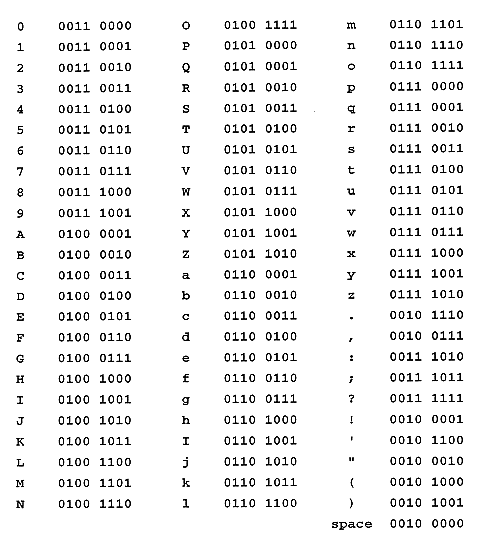
\includegraphics[width=0.8\linewidth]{ascii-binary-chart}
\caption{ASCII}
\end{figure}

Given its basic alphabet and importance for computing, binary has become the universal standard for understanding and communicating information.

\section{A Neatly Layered and Standardized System}

Although the idea of encoding information into a binary alphabet is incredibly well understood nowadays, the notion of binary had not been divined when Morse code was developed. Yet as we have seen, Morse code had its own pared down alphabet, lending evidence to assertion that simple alphabets with a small number of symbols tend to be naturally useful:

\begin{center}
\begin{tabular}{cc}
\thickdot & dot \\
\hline
\thickdash & dash \\
\hline
[short pause] & letter space \\
\hline
[long pause] & word space \\
\end{tabular}
\end{center}

Morse's alphabet was four symbols, and the translation of all information to and from this four-symbol alphabet is what makes the telegraph a \emph{digital} technology. A better word to describe the nature of the technology might be \emph{symbolic}; as we've seen, though, any symbolic alphabet can be encoded as digits, and so the word \emph{digital} is often used nowadays to refer to technologies that operate on discrete sets of symbols, as the telegraph did.

As a digital technology, the telegraph had to wrestle with many of the same questions that the Internet still wrestles with: how is digital information to be encoded and decoded? How will the process be standardized? Who will control the standardization process?

To begin with, the telegraph in contemporary parlance can be conceived of as a \emph{layered communication system}. In such a system, a single communication can be simultaneously described and thought about at different levels.

For example, suppose you are sending some message to your friend Bill via telegram. Another perfectly valid description at a lower level would be that a series of dots and dashes is being sent over telegraph wires between operators. At the lowest level, we find yet another description: electrical circuits manipulated by humans turn off and on in rapid succession.

The fact that electrical signals are being used to encode dots and dashes which in turn are being used to encode English letters allows us to form a nice mental picture of the layers of the system:

[DIAGRAM :
A. The physical layer of the electrical signal sent over the wire.

B. The translation of “signal on” and “signal off” into a very simple alphabet of dots, dashes, and spaces.

C. A translation of the simple alphabet of dots and dashes into the 26-letter alphabet (or more if we include extra characters such as spaces and special characters '?') of the English language.

D. A set of standards and abbreviations that telegraph operators used to communicate. For example, there is a standard shortcut for asking someone to retransmit a message [WRITE MORE ABOUT ITU?]
]

Thinking about communication technology as a layered system allows us to break down the system into component parts. Having built our communication system in this fashion, layers of the system can now be changed without changing everything all at once. For example, suppose there was an improvement to Morse code that was proven to be a more efficient translation of dots and dashes into the Latin alphabet. Then layer C above could be changed, but nothing else would have to change; you wouldn't need to invent new electrical gizmos to transmit or receive messages. Conversely, suppose the technology for the physical layer vastly improved and electricity were replaced with a more advanced technology like optical fibers. In this case, we could still use Morse code if we wanted, and so layers B-D would be unperturbed by changes in layer A.

\subsection{Metadata}

Let's take the time to be precise and think through what the systems for layer D might look like with respect to the telegraph.

Suppose you are a telegraph operator sitting in a local telegraph station in Idaho in the 1880s, and you are handed a telegram to transmit. It is identified as being from ``John Smith'' and going to a ``Mary Fitzpatrick'' along with a London address for the recipient. What steps do you have to take to deliver your telegram?

First, you have to decide how you are going to route your communication. Let's suppose there is a telegraph line from your local station to a central hub in New York City, which you know has a line directly to London.

So you hop on the line going to New York, and it is time to transmit the message. But wait – you have to convey information about the message as well as the message itself, such as the name and address of the recipient. This information about the message is known as metadata, because it is information about the message (in this parlance, the message is the “data”), as opposed to the message itself.

How does this metadata gets communicated? If you start tapping away at your telegraph key, do you start with the message itself? Or the metadata? Which piece of metadata? The location, maybe? The name of the recipient? That of the sender? Or perhaps some other boilerplate indicating “I have a new transmission for you”?

If you had all day to fumble through communicating this one telegram, you might be able to figure all of this out as you went, but if one is transmitting hundreds of telegrams per day, some sort of system is clearly needed. The system is represented by layer D above.

\subsection{Protocols}

The idea of system has a technical term in telecommunications – it is called a protocol. A protocol is a formal, agreed-upon system for communicating. In this case, the telegraph community uses a protocol for message transmission to avoid any ambiguity about the what information is metadata (e.g. the name of the sender) vs data (i.e. the contents of the message).

You can think of the rules of driving cars on public streets as a protocol. We drive on the right side of the road in the United States. It doesn't particularly matter that we chose the right instead of the left, and other countries have chosen differently. What matters is that we make one choice or the other and stick to it, else each time two cars approached each other on the road, they would have to improvise an ad hoc solution.

Protocols exist to enforce this consistency and establish an agreed upon standard for the interaction of two or more agents.

As we will see when we explore the rise of the Internet later in the book, establishing some open, universal standard protocol is quite often much more advantageous to a situation in which there are competing fiefdoms each using their own protocol.

Yet while the importance of a universal standard is critical, it is also important to note that there is often quite a lot of debate when designing and standardizing protocols. Good protocols are simple and efficient, but there are often trade offs and no clear ``best'' protocol in any given situation. Different stakeholders may have different requirements and different preferences in how a protocol is designed. Moreover, once a protocol is standardized, it can become quite entrenched, and so many people and entities have to live with it a while, increasing the importance of getting it as agreeable as possible the first time.

We will revisit these ideas of layered systems, protocols, and metadata extensively later when we learn about the Internet and the systems of communication of which it is comprised. That global system is much more complex, but fortunately, the telegraph as a digital technology in its own right provides us with a gentle introduction.

\section{Encryption}

Unlike Chappe's optical telegraph, which was strictly intended for military use, electrical telegraphy thrived because it was embraced by the private sector. Companies quickly saw the value of investing in telegraph infrastructure and then charging for communications sent over their networks.

At first there was an explosion of competition. By 1851, a mere 7 years after Morse's first successful long distance demonstration, there were already 75 companies operating in the United States that had laid over 21,000 miles of telegraph cable [CITE: https://eh.net/encyclopedia/history-of-the-u-s-telegraph-industry/]. However, telecommunications benefit tremendously from economies of scale. Why build two separate lines in competition between New York and Chicago? That leads to wasteful duplication of effort in laying cables, building telegraph offices, and so forth. Thus, economic pressure over the next 15 years pushed the industry towards consolidation, and by 1866 Western Union emerged as the dominant national telegraph monopoly.

The cost of sending a domestic telegram varied quite a bit, but during the first twenty or thirty years, it was cost-prohibitive as a regular means of communication to all except businesses and wealthy individuals. For example, in 1860, the cost of a ten word telegram from New York to New Orleans cost $2.70, or about $70 in 2014 dollars. Using the Transatlantic lines was much more expensive, costing about $100 at the time for a telegram to England, or $2600 in 2014 dollars. [CITE: http://www.gizmag.com/last-telegraph-message/28314/]

Given the high cost of sending telegrams and the fact that companies like Western Union charged by the word, people learned to be creatively brief with their messages. At first this was ad hoc, but by the mid 1800s, code books were developed and published that aimed to translate common phrases into single words, saving money for the users of the telegraph network. This also made the network itself more efficient at moving information around. Indeed, when code words were used, the dots and dashes had a higher information density than they would typing out the full English phrase, a notion that we will make precise in coming chapters.

To get a sense of the code books, here is an excerpt from  [INSERT FROM]

[INSERT EXCERPT]

Notice that this is also a type of encoding just as we saw earlier, this time from the alphabet of a limited set of phrases into an alphabet of special words intended for use in telegraphy.

\subsection{Encryption}

These telegraph code books helped people communicate more efficiently, saving them money, but sometimes it was not cost savings but rather the privacy of the message that was the paramount concern. Since these telegraphy code books were for the most part not secret, anyone could decode a message written using this telegraphy code simply by consulting the relevant publicly available code book.

Protecting the secrecy of your message, on the other hand, meant \emph{encrypting} it. Encryption is a general term that refers to the process of scrambling a message with the goal of making it unreadable to anyone except the intended recipient. Encryption has been around for thousands of years, and so it was natural to apply existing techniques to telegraphy.

How did it actually work? Let's suppose you had to send a message overseas and you wanted it to be secret. One method might be to replace each letter in the alphabet with another equivalent: so 'A' becomes 'T', 'B' becomes 'H' and so on. According to this scheme, the sentence:

   \[ 'BATS CANNOT SEE' \]

Might become

   \[ 'HTQY VTBBJQ YRR' \]

Let's pause to introduce a bit of jargon. In the case above, the original message written in English is called the \emph{plaintext}. The scheme for moving from the plaintext to its encrypted form is called a \emph{cipher}, and the encrypted text is called the \emph{ciphertext}. Going from the plaintext to the ciphertext is \emph{encryption} and going from the ciphertext back to the plaintext is called \emph{decryption}.

For this example, you encrypt and decrypt using the mapping that we created:

\begin{align*}
	\text{'A'} &-> \text{'T'} \\
	\text{'B'} &-> \text{'H'} \\
	\text{'C'} &-> \text{'V'} \\
        \text{etc}
\end{align*}

This short mapping is called the \emph{encryption key}. And notice that it also works as the decryption key, and so in the context of ciphers can just be called the \emph{key}. It ought to work somewhat like a physical key: if you possess the key, then you can read the plaintext, otherwise you are out of luck.

Since the same key is used for both encryption and decryption, we say that this scheme is \emph{symmetric}, and the particular cipher we have described is known as a simple substitution cipher.

This is a good first pass, but as you might imagine, simple substitution ciphers tend to be a rather weak form of encryption. Let's now switch gears and put ourselves in the mind of an attacker. How could we break this encryption? To add just one last piece of jargon, if one is attempting to break the encryption of a message without having the key, that is known as \emph{cryptanalysis}. Your first instinct might be to try every possible key until you get a message that is an English sentence. This is known as a brute force attack.

How many keys would you have to try? To compute this, notice that the letter 'A' must be mapped to one of 26 letters (allowing the mapping 'A' → 'A'). So there are 26 possibilities for 'A'. Once we have fixed 'A', how many possibilities are there for 'B'. Well, 'A' and 'B' cannot both map to the same letter (in other words 'A'->'D', 'B'->'D' is not a valid key). This means that once 'A' is fixed, there is one less option for 'B', giving a total of 25 possibilities for 'B'. Having fixed both 'A' and 'B' there are 24 possibilities for C. If we continue in this way, we can see that the total number of keys is

\[ 26*25*24*23* … * 2 * 1 \]

There is a mathematical abbreviation for this term: 26! (the exclamation point is an operator called \emph{factorial}).

This turns out to be a surprisingly large number:

\[ 403291461126605635584000000 \]

Of course we may not need to check every single key. After all, we might get lucky and find the correct key early on. We can express this in terms of probability. Assuming the key was chosen randomly, so that all keys are equally likely, each key has a

\[ 1/403291461126605635584000000 \]

of being the correct one. This means that it is astronomically unlikely that we will get the correct key after just one or two tries. Even a million attempts gives us a probability of

\[ 1000000/403291461126605635584000000 \]

of finding the right key. This is way too small for us to bank on. If we wanted to get to a 50% chance of finding the key via our brute force method, we would need to expect to have to try

\[ 403291461126605635584000000/2 \]

possibilities. Using more standard exponential notation for large numbers, we can say that this is about $2*10^{26}$. That may seem like a lot, but well within reach for an average computer nowadays.

Unfortunately if you were trying to decrypt ciphertext in the 1860s without the key, you didn't have computers at your disposal to help perform some enormous amount of operations. So given that a brute force attack seems infeasible without a lot of computational assistance, how else might we try to decrypt a message encrypted with a simple substitution cipher? The main technique to employ is called \emph{frequency analysis} which is based on the observation that English letters are not randomly distributed in words. 'e' occurs more frequently than 'q' or 'z'. It also helps that you know the length of each word since the simple substitution cipher does not change word lengths. In the example above, the ciphertext of the last word is 'YRR'. There are only 43 three-letter words in the Scrabble dictionary that have this form, giving us a ton of information and significantly cutting down on the number of possibilities we have to check compared to our brute force approach. Armed with techniques like these, after studying a ciphertext for some length of time, one can usually start to slowly recover messages piece by piece like a Sudoku puzzle.

Of course, people designing encryption systems were creative too, and came up with schemes far more complex than simple substitution ciphers. Perhaps the most famous encrypted telegram was the so-called Zimmermann Note which was sent by the German Foreign Office in 1917 to the German Ambassador to Mexico instructing the latter to propose a military alliance between Germany and Mexico should the United States enter World War I.

Here is the ciphertext of this infamous telegram as it appears on the telegram:

\begin{figure}[H]
\centering
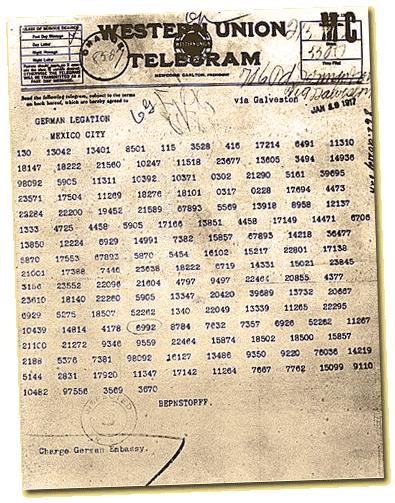
\includegraphics[width=0.8\linewidth]{zimmermann}
\caption{Zimmermann Note}
\end{figure}

This message is encrypted with a cipher named ``cipher 0075'', which is of course much more complicated than a simple substitution cipher. Yet the British had a crack team of codebreakers throughout both World Wars – known as Room 40 – and were able to apply more advanced versions of the techniques we saw above in order to break the cipher. When the Germans' clandestine proposal was revealed, Americans were outraged and this was one of the major tipping points that pulled the United States into World War I.

\end{CJK}
\end{document}
